
\chapter{Cadre général du projet}
\label{chap:cadre_general}

% ============================================================
\section*{Introduction}
\addcontentsline{toc}{section}{Introduction}

Ce chapitre a pour objectif de présenter le cadre général dans lequel s'inscrit ce projet
de fin d'études. Nous commençons par une présentation de l'organisme d'accueil, puis
nous effectuons une étude de l'existant afin d'identifier les lacunes des solutions actuelles
de surveillance des systèmes SAP. Nous détaillons ensuite la problématique retenue, avant
de présenter la solution proposée et la méthodologie de développement adoptée.

% ============================================================
\section{Présentation de l'organisme d'accueil}
\label{sec:organisme}

\subsection{AVAXIA GROUP}

AVAXIA GROUP est une société de conseil en technologies de l'information à dimension
internationale, fondée en 2006. Elle dispose d'une présence stratégique dans plusieurs
régions, avec son siège social à Dubaï et des centres opérationnels en Tunisie, au Japon
et au Canada. L'organisation est spécialisée dans les solutions technologiques d'entreprise,
avec un accent particulier sur l'implémentation des systèmes ERP (\textit{Enterprise Resource
Planning}), l'intégration de systèmes et les services gérés pour les applications métiers
critiques. Son expertise technique s'étend à l'écosystème SAP ainsi qu'à des plateformes
complémentaires telles que Salesforce.

\begin{figure}[htbp]
  \centering
  
\includegraphics[width=0.35\textwidth]{avaxia_logo.png}

  \caption{Logo Avaxia Group}
  \label{fig:avaxia_logo.png}
\end{figure}

\subsection{Philosophie et approche}

Avaxia Group adopte une méthodologie résolument centrée sur le client dans son modèle
de prestation de services, en privilégiant des partenariats collaboratifs plutôt que des
relations purement transactionnelles.

\subsection{Portefeuille de services}

Avaxia met à disposition  un portefeuille complet de services numériques et de conseil, avec une
forte orientation vers les solutions d'entreprise, le support d'infrastructure et les
technologies émergentes. Le groupe est structuré autour de deux départements spécialisés,
chacun offrant des domaines de services distincts :

\begin{itemize}[leftmargin=*, label=\textbullet]
  \item \textbf{Consultance fonctionnelle :} Conception de solutions métier pour le
        déploiement de nouveaux modules SAP fonctionnels, analyse et optimisation des
        processus de bout en bout, ainsi que la gestion du déploiement fonctionnel et de
        la planification des tests.
  \item \textbf{Big Data :} Services incluant la gestion, la transformation, l'intégration,
        le stockage et l'analyse des données. Les compétences couvrent le développement de
        pipelines de données, les processus ETL et la gouvernance des données.
  \item \textbf{VR / AR :} Développement d'environnements VR interactifs permettant aux
        utilisateurs de naviguer, d'interagir avec des objets et de collaborer en temps
        réel. Les applications comprennent les systèmes de surveillance, les simulations,
        les programmes de formation et les visites virtuelles.
\end{itemize}

\subsection{Structure organisationnelle}

L'architecture organisationnelle d'Avaxia Group est conçue pour faciliter une expertise
spécialisée tout en maintenant une collaboration transversale. La structure du groupe
s'articule autour de trois niveaux :

\begin{itemize}[leftmargin=*, label=\textbullet]
  \item \textbf{Organisation divisionnelle :} Assure les responsabilités de chaque
        département en fonction de son rôle, en gérant le développement commercial et les
        décisions stratégiques.
  \item \textbf{Organisation opérationnelle :} Se concentre sur les défis techniques et
        les expertises qui pilotent les projets et services (planification, exécution,
        livraison et support). Elle permet également de suivre, évaluer et optimiser les
        opérations de projets.
  \item \textbf{Structure corporative :} Supporte le front office en représentant les
        opérations internes (Finance, RH, Formation, Marketing, Qualité de service,
        Informatique), afin d'assurer la continuité de l'activité dans son ensemble.
\end{itemize}

Ce projet se déroule au sein de l'équipe Quadient, rattachée au département
\textit{SAP Infrastructure and BASIS} du bureau tunisien d'Avaxia Group. Les
responsabilités de cette équipe englobent la surveillance et le support des systèmes SAP
critiques auprès de plusieurs clients, ce qui en fait un environnement idéal pour
développer et valider un système avancé de détection d'anomalies basé sur la technologie
RAG.

% ============================================================
% ============================================================
\section{Étude de l'existant}
\label{sec:existant}

Dans le cadre du développement d’un système intelligent de surveillance des systèmes SAP
au sein d’Avaxia Group, une étude de l’existant a été réalisée afin de comprendre les
processus actuels mis en œuvre par l’équipe BASIS.

\subsection*{Rôle du consultant SAP BASIS}

Le consultant SAP BASIS est responsable de l’administration technique des systèmes SAP.
Ses missions principales incluent la surveillance des systèmes, la gestion des performances,
le traitement des incidents techniques ainsi que la maintenance quotidienne des environnements SAP.

Dans le cadre de la surveillance, le consultant BASIS vérifie régulièrement l’état global
du système à travers différentes transactions SAP. Il analyse les jobs en arrière-plan,
les erreurs système, les impressions en attente ainsi que l’activité des processus.
Ces actions permettent d’assurer le bon fonctionnement des systèmes et d’identifier
les anomalies éventuelles.
\subsection*{Surveillance des systèmes SAP}

La surveillance quotidienne des systèmes SAP repose sur l’utilisation de plusieurs codes
de transaction (T-codes), chacun fournissant des informations spécifiques :

\begin{itemize}
    \item \texttt{SM37} : permet de consulter les jobs en arrière-plan et leur état d’exécution.
    \item \texttt{ST22} : permet d’analyser les dumps ABAP générés par les erreurs système.
    \item \texttt{SP01} : permet de visualiser les spools d’impression.
    \item \texttt{DB02} : fournit des informations sur l’état de la base de données.
    \item \texttt{SM66} : permet de superviser les processus actifs du système.
\end{itemize}

Ces transactions sont utilisées de manière régulière par les consultants BASIS afin de
collecter les informations nécessaires à la supervision des systèmes SAP.
% ============================================================
% Schema 1 : Surveillance manuelle des systèmes SAP
% ============================================================
\begin{figure}[H]
\centering
\begin{tikzpicture}[
    node distance=0.8cm,
    every node/.style={font=\small},
    mainbox/.style={draw, rounded corners=4pt, minimum height=0.9cm, text centered, font=\small\bfseries},
    tcode/.style={draw=#1, fill=#1!10, rounded corners=4pt, minimum width=2.2cm, minimum height=1.2cm, text centered, font=\small\bfseries, text=#1!80!black},
    resultbox/.style={draw=red!70!black, fill=red!5, rounded corners=4pt, minimum height=0.9cm, text centered, font=\small\bfseries, text=red!70!black},
    arr/.style={-{Stealth[length=5pt]}, thick, color=gray!70!black},
]

% Consultant
\node[mainbox, draw=blue!60, fill=blue!8, minimum width=5cm] (consultant) {Consultant BASIS};

% Daily check
\node[mainbox, draw=gray!60, fill=gray!8, minimum width=7cm, below=of consultant] (check) {Vérification manuelle quotidienne};
\draw[arr] (consultant) -- (check);

% Annotation
\node[font=\scriptsize\itshape, color=gray!70, below=0.15cm of check] (annot) {Interroge chaque T-code séparément};

% T-codes row
\node[tcode=violet, below=1cm of check, xshift=-5cm] (sm37) {\textbf{SM37}\\\scriptsize Jobs batch};
\node[tcode=violet, right=0.3cm of sm37] (st22) {\textbf{ST22}\\\scriptsize Dumps ABAP};
\node[tcode=violet, right=0.3cm of st22] (sp01) {\textbf{SP01}\\\scriptsize Spools};
\node[tcode=violet, right=0.3cm of sp01] (db02) {\textbf{DB02}\\\scriptsize Stats BD};
\node[tcode=violet, right=0.3cm of db02] (sm66) {\textbf{SM66}\\\scriptsize Processus};

% Arrows from check to T-codes
\foreach \n in {sm37, st22, sp01, db02, sm66} {
    \draw[arr] (check.south) -- ++(0,-0.3) -| (\n.north);
}

% Convergence
\coordinate (conv) at ($(sp01.south)+(0,-0.8)$);
\foreach \n in {sm37, st22, sp01, db02, sm66} {
    \draw[gray!50, thin] (\n.south) -- (\n.south |- conv);
}
\draw[gray!50, thin] (sm37.south |- conv) -- (sm66.south |- conv);

% Manual analysis
\node[mainbox, draw=orange!70!black, fill=orange!8, minimum width=7cm, below=1.5cm of sp01, text=orange!70!black] (analyse) {Analyse manuelle};
\node[font=\scriptsize\itshape, color=gray!60, below=0.05cm of analyse] {Sans agrégation $\cdot$ Risque d'omission};
\draw[arr] (conv) -- (analyse.north);

% Result
\node[resultbox, minimum width=5.5cm, below=0.8cm of analyse] (result) {Détection tardive des anomalies};
\draw[arr] (analyse.south) -- (result.north);

\end{tikzpicture}
\caption{Processus de surveillance manuelle des systèmes SAP}
\label{fig:surveillance-manuelle}
\end{figure}

\subsection*{Structure des données SAP}

Les systèmes SAP génèrent quotidiennement un volume important de données sous forme de logs.
Chaque transaction produit des informations selon une structure spécifique.

Par exemple :
\begin{itemize}
    \item \texttt{SM37} expose des champs tels que \textit{Job\_Name}, \textit{Job\_ID},
    \textit{Status}, \textit{Start\_Date} et \textit{End\_Date}.
    \item \texttt{ST22} fournit des informations comme \textit{Error\_Name},
    \textit{Server}, \textit{Date}, \textit{Time}, \textit{User} et \textit{Client}.
    \item \texttt{SP01} contient des données telles que \textit{Spool\_Number},
    \textit{Owner}, \textit{Created\_On} et \textit{Status}.
\end{itemize}

Ces données sont utilisées par les consultants pour analyser l’état du système et suivre
les différentes activités en cours.
% ============================================================
% Schema 2 : Surcharge et hétérogénéité des données
% ============================================================
\begin{figure}[H]
\centering
\begin{tikzpicture}[
    node distance=0.8cm,
    every node/.style={font=\small},
    mainbox/.style={draw, rounded corners=4pt, minimum height=0.9cm, text centered, font=\small\bfseries},
    fieldbox/.style={draw=#1!40, fill=#1!4, rounded corners=4pt, minimum width=3.8cm, minimum height=3.5cm, text centered, align=center},
    resultbox/.style={draw=red!35, fill=red!3, rounded corners=4pt, minimum height=1.1cm, text centered, align=center, minimum width=3.8cm},
    arr/.style={-{Stealth[length=5pt]}, color=gray!50},
]
 
% SAP System
\node[mainbox, draw=gray!35, fill=gray!4, minimum width=12cm] (sap) {Système SAP --- volume important de logs quotidiens};
 
% SM37
\node[fieldbox=blue!30, below=1cm of sap, xshift=-4.5cm] (sm37) {};
\node[font=\small\bfseries, text=blue!45!black] at ($(sm37.north)+(0,-0.4)$) {SM37};
\node[font=\scriptsize\itshape, text=gray!55] at ($(sm37.north)+(0,-0.75)$) {Jobs en arrière-plan};
\node[font=\scriptsize\ttfamily, text=gray!60, anchor=west, align=left] at ($(sm37.west)+(0.3,-0.3)$) {
    Job\_Name\\Job\_ID\\Status\\Start\_Date\\End\_Date
};
 
% ST22
\node[fieldbox=teal!35, below=1cm of sap] (st22) {};
\node[font=\small\bfseries, text=teal!45!black] at ($(st22.north)+(0,-0.4)$) {ST22};
\node[font=\scriptsize\itshape, text=gray!55] at ($(st22.north)+(0,-0.75)$) {Dumps ABAP};
\node[font=\scriptsize\ttfamily, text=gray!60, anchor=west, align=left] at ($(st22.west)+(0.3,-0.3)$) {
    Error\_Name\\Server\\Date, Time\\User\\Client
};
 
% SP01
\node[fieldbox=orange!20, below=1cm of sap, xshift=4.5cm] (sp01) {};
\node[font=\small\bfseries, text=orange!45!black] at ($(sp01.north)+(0,-0.4)$) {SP01};
\node[font=\scriptsize\itshape, text=gray!55] at ($(sp01.north)+(0,-0.75)$) {Spools d'impression};
\node[font=\scriptsize\ttfamily, text=gray!60, anchor=west, align=left] at ($(sp01.west)+(0.3,-0.3)$) {
    Spool\_Number\\Type\\Owner\\Created\_On\\Status
};
 
% Arrows from SAP to T-codes
\foreach \n in {sm37, st22, sp01} {
    \draw[arr] (sap.south) ++(0,0) -- ++(0,-0.2) -| (\n.north);
}
 
% Dashed warning zone
\node[draw=red!35, dashed, rounded corners=6pt, fill=red!2,
      minimum width=13cm, minimum height=1.3cm,
      below=0.8cm of st22.south, align=center] (noagg) {
    {\bfseries\color{red!45!black} Aucun mécanisme d'agrégation unifié}\\[-1pt]
    {\scriptsize\itshape\color{red!35!black} Structures variables traitées séparément}
};
 
\foreach \n in {sm37, st22, sp01} {
    \draw[arr] (\n.south) -- (\n.south |- noagg.north);
}
 
% Consequences
\node[resultbox, below=0.8cm of noagg, xshift=-3cm] (frag) {
    {\bfseries\color{red!45!black} Analyse fragmentée}\\[-1pt]
    {\scriptsize\itshape\color{gray!60} Corrélation impossible}
};
\node[resultbox, below=0.8cm of noagg, xshift=3cm] (surcharge) {
    {\bfseries\color{red!45!black} Surcharge cognitive}\\[-1pt]
    {\scriptsize\itshape\color{gray!60} Risque d'erreur humaine}
};
 
\draw[arr] (noagg.south) ++(0,0) -- ++(0,-0.15) -| (frag.north);
\draw[arr] (noagg.south) ++(0,0) -- ++(0,-0.15) -| (surcharge.north);
 
\end{tikzpicture}
\caption{Surcharge et hétérogénéité des données issues des T-codes SAP}
\label{fig:heterogeneite-donnees}
\end{figure}


\subsection*{Gestion de la connaissance SAP}

La connaissance SAP au sein de l'équipe est répartie entre plusieurs sources : le portail
SAP Help, qui organise la documentation de manière hiérarchique sur des milliers de
pages, des livres techniques au format PDF, des SAP Notes référencées par numéro, et
l'expérience individuelle des consultants. Chaque consultant accède à ces sources de
manière indépendante selon ses besoins, sans système centralisé de partage ou de
capitalisation des connaissances.
% ============================================================
% ============================================================
\subsection{Critique de l'existant}
\label{sec:critique}

L’analyse de l’existant met en évidence plusieurs limites structurelles et
fonctionnelles dans les processus actuels de surveillance et de gestion de la
connaissance au sein de l’équipe BASIS.

\subsubsection*{Limites de la surveillance des systèmes SAP}

Le processus actuel de surveillance repose principalement sur une approche manuelle,
dans laquelle les consultants BASIS interrogent individuellement plusieurs transactions
afin d’obtenir une vision de l’état du système. Cette approche induit une dépendance
forte à l’intervention humaine et mobilise un effort opérationnel important, notamment
dans des environnements multi-systèmes.

En outre, l’absence de consolidation des informations issues des différents T-codes
ne permet pas d’obtenir une vue globale et cohérente du système. Les données étant
consultées de manière isolée, la corrélation entre événements devient difficile,
ce qui limite la capacité d’analyse transversale.

Par ailleurs, le mode de surveillance actuel repose sur des mécanismes de détection
basés sur des seuils statiques. Ce type d’approche présente des limites importantes :
d’une part, il peut générer un volume élevé d’alertes non pertinentes dans le cas
de variations normales du système ; d’autre part, certaines anomalies progressives
ou atypiques peuvent ne pas être détectées si elles ne dépassent pas les seuils définis.

Enfin, l’absence de mécanismes d’analyse prédictive ou de détection des tendances
empêche toute anticipation des dégradations du système, limitant ainsi la surveillance
à une logique essentiellement réactive.

\subsubsection*{Limites liées à la gestion des données}

Les données générées par les systèmes SAP présentent une forte hétérogénéité en termes
de structure et de format, chaque transaction produisant ses propres champs et
indicateurs. Cette diversité complique leur exploitation et rend difficile toute
forme de traitement unifié.

L’absence d’un mécanisme d’agrégation ou de normalisation des données limite la
possibilité d’analyse globale et empêche la mise en place d’outils avancés d’analyse,
notamment dans le cadre de la détection d’anomalies ou de corrélations complexes entre événements.

De plus, le volume important de données à analyser quotidiennement constitue une
charge cognitive significative pour les consultants, ce qui peut impacter l’efficacité
du processus de surveillance et la rapidité de prise de décision.

\subsubsection*{Limites de la gestion des connaissances SAP}

La gestion des connaissances au sein de l’équipe repose sur un ensemble de sources
hétérogènes et distribuées, incluant la documentation officielle, les SAP Notes
et les ressources internes. Cette organisation ne repose sur aucun système unifié
permettant une centralisation ou une structuration des informations.

La recherche d’information s’effectue généralement à partir de mots-clés, sans prise
en compte du contexte sémantique ni des relations entre les documents. Cela peut
entraîner des difficultés dans l’identification rapide des informations pertinentes.

Par ailleurs, les liens entre les différentes منابع documentaires ne sont pas
explicitement structurés, ce qui oblige les consultants à naviguer manuellement entre
plusieurs sources. Cette situation peut allonger les délais de résolution des incidents.

Enfin, la dépendance à l’expertise individuelle constitue un facteur de fragilité
organisationnelle. L’absence de mécanismes de capitalisation et de partage structuré
des connaissances peut entraîner une perte d’information critique en cas d’indisponibilité
ou de départ de certains experts.
\subsection{Solutions existantes et analyse concurrentielle}
\label{sec:solutions_existantes}

Plusieurs solutions dédiées ou adaptées à la surveillance des environnements SAP
existent actuellement. Ces solutions se distinguent principalement par leur niveau
d’intégration avec l’écosystème SAP, leurs capacités d’analyse ainsi que leur
approche de la détection des anomalies.

\subsubsection*{Outils natifs SAP}

Les outils natifs proposés par SAP constituent la première catégorie de solutions
utilisées pour la supervision des systèmes. Parmi eux, SAP Solution Manager (SolMan)
offre un ensemble de fonctionnalités intégrées permettant la surveillance technique,
la gestion des incidents ainsi que le suivi des performances des systèmes SAP.

Cette solution présente l’avantage d’une intégration native avec les environnements SAP,
permettant un accès direct aux données internes et aux transactions. Elle propose
également des mécanismes de monitoring centralisé et des outils de diagnostic.

Cependant, ces outils restent principalement orientés vers une surveillance technique
classique. Ils reposent en grande partie sur des règles et des seuils prédéfinis,
et offrent des capacités limitées en matière d’analyse intelligente, notamment en
ce qui concerne la détection proactive des anomalies ou l’interprétation contextuelle
des événements.

\subsubsection*{Solutions SAP basées sur le Machine Learning}

SAP propose également des solutions intégrant des capacités de Machine Learning,
notamment à travers SAP Leonardo ML. Ces solutions permettent d’exploiter les données
générées par les systèmes SAP afin d’identifier des patterns et de détecter certaines
anomalies.

L’intégration native avec les systèmes ERP constitue un avantage majeur, facilitant
l’accès aux données et leur traitement en temps réel. Ces outils permettent également
d’introduire une dimension prédictive dans la surveillance des systèmes.

Néanmoins, ces solutions présentent certaines limites, notamment en termes de flexibilité
et de personnalisation. Elles sont généralement dépendantes de l’écosystème SAP et
souvent orientées vers des déploiements cloud, ce qui peut ne pas convenir à toutes
les architectures existantes. De plus, leur coût peut représenter un frein pour
certaines organisations.

\subsubsection*{Approches hybrides et pratiques courantes}

En complément des outils existants, de nombreuses organisations adoptent des approches
hybrides combinant les outils SAP avec des procédures manuelles réalisées par les
consultants BASIS. Ces pratiques incluent l’utilisation des T-codes de surveillance
ainsi que l’analyse directe des logs système.

Cette approche permet une certaine flexibilité et une adaptation aux besoins spécifiques
de chaque environnement SAP. Elle repose toutefois fortement sur l’expertise humaine
et nécessite une interprétation manuelle des informations collectées.
\subsubsection*{Synthèse comparative}

\begin{table}[H]
\centering
\caption{Synthèse des solutions de surveillance SAP}
\label{tab:synthese_sap}
\renewcommand{\arraystretch}{1.4}
\begin{tabular}{|p{3.2cm}|p{3.5cm}|p{3.5cm}|p{3.5cm}|}
\hline
\textbf{Catégorie} & \textbf{Approche} & \textbf{Points forts} & \textbf{Limites} \\
\hline

Outils natifs SAP (SolMan)
&
Surveillance basée sur T-codes et règles prédéfinies
&
Intégration native avec SAP \newline
Accès direct aux données système \newline
Supervision centralisée
&
Faible capacité d'analyse intelligente \newline
Basé sur des seuils statiques \newline
Peu flexible
\\
\hline

Solutions SAP avec Machine Learning (SAP Leonardo ML)
&
Analyse basée sur des modèles de Machine Learning
&
Détection d'anomalies \newline
Analyse prédictive \newline
Intégration ERP native
&
Coût élevé \newline
Dépendance au cloud \newline
Personnalisation limitée
\\
\hline

Approches hybrides (outils + intervention humaine)
&
Combinaison de monitoring automatique et analyse manuelle
&
Flexibilité \newline
Adaptation aux besoins spécifiques \newline
Exploitation de l'expertise humaine
&
Dépendance aux consultants \newline
Charge opérationnelle élevée \newline
Risque d'erreur humaine
\\
\hline

\end{tabular}
\end{table}
\subsubsection*{Synthèse}

L’analyse des solutions existantes montre que, malgré la disponibilité d’outils
performants, la surveillance des systèmes SAP reste largement dépendante de
configurations spécifiques, de règles statiques et de l’intervention humaine.

Les capacités d’analyse avancée, notamment en termes de compréhension contextuelle
des événements et de détection intelligente des anomalies, restent limitées ou
partiellement exploitées dans les solutions actuelles.
\label{sec:solution}

Afin de remédier aux limites constatées dans le système actuel, un système de surveillance
intelligent des environnements SAP est proposé. Cette solution a pour objectif d'automatiser
la détection des anomalies, de fournir des alertes enrichies en contexte et de centraliser
l'accès à la documentation SAP.


\begin{itemize}[leftmargin=*, label=\textbullet]

  \item \textbf{Collecte et traitement de la documentation :} La solution collecte automatiquement
la documentation SAP depuis le portail SAP Help ainsi que les livres techniques, en
préservant leur structure et leur contenu. Les données collectées sont ensuite nettoyées,
organisées et enrichies avec des informations contextuelles pour faciliter leur
exploitation ultérieure.

  \item \textbf{Collecte et traitement de la documentation :} La solution collecte automatiquement
la documentation SAP depuis le portail SAP Help ainsi que les livres techniques, en
préservant leur structure et leur contenu. Les données collectées sont ensuite nettoyées,
organisées et enrichies avec des informations contextuelles pour faciliter leur
exploitation ultérieure.

  \item \textbf{Base de connaissances centralisée :} L'ensemble de la documentation traitée est
stocké dans une base de connaissances unifiée, permettant aux consultants d'interroger
directement le système en langage naturel pour retrouver une information pertinente, sans
avoir à naviguer manuellement entre plusieurs sources.



  \item \textbf{Recherche et génération de réponses :} Lorsqu'un consultant pose une question,
le système identifie les documents les plus pertinents dans la base de connaissances et
génère automatiquement une réponse argumentée et sourcée, adaptée au contexte de la
requête.
  \item \textbf{Prévention des erreurs :} Des mécanismes de validation sont intégrés pour
s'assurer que les réponses générées sont bien fondées sur la documentation disponible
et non sur des informations incorrectes.
  \item \textbf{Interface et déploiement :} La solution est accessible via une interface web
intuitive comprenant un chatbot de support, un tableau de bord de surveillance en temps
réel et un panneau d'administration. Elle est également connectée à Microsoft Teams afin
de notifier automatiquement les équipes lors de la survenue d'incidents critiques.




\end{itemize}

% ============================================================
\section{Méthodologie de développement}
\label{sec:methodologie}


\subsection{Présentation des méthodologies candidates}

\subsubsection{CRISP-DM}

CRISP-DM (\textit{Cross-Industry Standard Process for Data Mining}) est une méthodologie
éprouvée par l'industrie pour guider les projets de fouille de données. Son cycle de vie
se compose de six phases interdépendantes (voir Figure~\ref{fig:crisp_dm}) :

\begin{figure}[htbp]
  \centering
   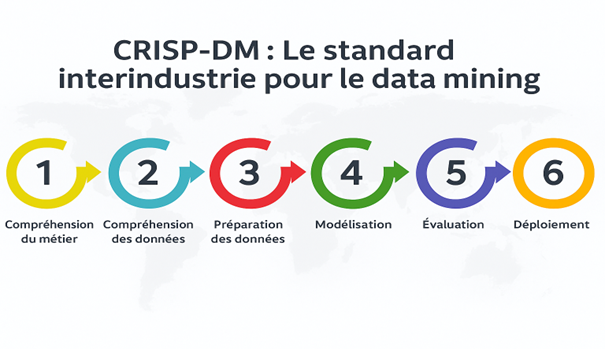
\includegraphics[width=0.65\textwidth]{crisp_dm.png}

  \caption{Cycle de vie du framework CRISP-DM}
  \label{fig:crisp_dm}
\end{figure}

\begin{enumerate}[leftmargin=*, label=\arabic*.]
  \item \textbf{Compréhension métier (\textit{Business Understanding}) :} Définir les
        objectifs du projet et traduire les objectifs métier en problèmes de fouille de
        données.
  \item \textbf{Compréhension des données (\textit{Data Understanding}) :} Collecter les
        données initiales, évaluer leur qualité et découvrir des premières perspectives.
  \item \textbf{Préparation des données (\textit{Data Preparation}) :} Nettoyer,
        transformer et mettre en forme les données pour les besoins de la modélisation.
  \item \textbf{Modélisation (\textit{Modeling}) :} Sélectionner et appliquer des
        techniques de modélisation avec des paramètres optimisés.
  \item \textbf{Évaluation (\textit{Evaluation}) :} Évaluer les résultats du modèle par
        rapport aux objectifs métier et aux critères de succès.
  \item \textbf{Déploiement (\textit{Deployment}) :} Mettre en production les résultats
        et établir une stratégie de surveillance continue.
\end{enumerate}

\paragraph{Avantages de CRISP-DM}
\begin{itemize}[leftmargin=*, label=\textbullet]
  \item \textbf{Orienté métier :} Démarre par la compréhension métier, en parfait
        alignement avec les besoins d'entreprise tels que l'interprétation des anomalies
        SAP et l'analyse d'impact.
  \item \textbf{Workflow itératif :} Encourage les retours continus et le raffinement du
        modèle, utile pour améliorer la précision et la pertinence des alertes.
  \item \textbf{Neutre technologiquement :} N'impose pas de contraintes d'outillage, bien
        adapté à une intégration flexible avec des stacks modernes.
  \item \textbf{Largement adopté :} Éprouvé par l'industrie et soutenu par une
        documentation et des outils abondants.
  \item \textbf{Accent sur l'évaluation :} Inclut des phases dédiées à l'évaluation de
        la performance technique et de l'adéquation métier, essentielles pour les
        applications de surveillance SAP.
\end{itemize}

\paragraph{Limites de CRISP-DM}
\begin{itemize}[leftmargin=*, label=\textbullet]
  \item \textbf{Absence de MLOps intégré :} Ne traite pas nativement les pratiques de
        déploiement modernes (CI/CD, versionnage, surveillance).
\end{itemize}

\subsubsection{KDD – Knowledge Discovery in Databases}

Le processus KDD (\textit{Knowledge Discovery in Databases}), introduit par Fayyad et al.
en 1996, est l'une des premières méthodologies formelles pour extraire des connaissances
actionnables de larges volumes de données. Il met l'accent sur le cycle de vie complet,
de la préparation des données jusqu'à l'interprétation des connaissances.

\begin{figure}[htbp]
  \centering
   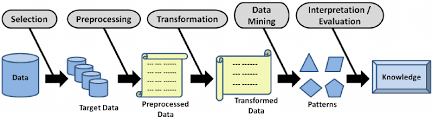
\includegraphics[width=0.65\textwidth]{kdd.png}

  \caption{Étapes du processus KDD}
  \label{fig:kdd}
\end{figure}

\paragraph{Avantages}
\begin{itemize}[leftmargin=*, label=\textbullet]
  \item Fort accent sur la validité, la nouveauté et l'utilité des connaissances.
  \item Promeut un pipeline d'analyse de données complet et itératif.
\end{itemize}

\paragraph{Inconvénients}
\begin{itemize}[leftmargin=*, label=\textbullet]
  \item Guidance limitée sur le déploiement ou l'opérationnalisation.
  \item Moins d'accent sur les pratiques agiles ou les principes d'ingénierie logicielle.
\end{itemize}

\subsubsection{TDSP – Team Data Science Process}

Le TDSP (\textit{Team Data Science Process}) est un framework développé par Microsoft
pour guider les projets de data science. Son cycle de vie comprend cinq étapes itératives,
similaires à celles de CRISP-DM (voir Figure~\ref{fig:tdsp}).

\begin{figure}[htbp]
  \centering
   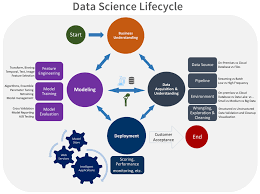
\includegraphics[width=0.65\textwidth]{tdsp (1).png}

  \caption{Cycle de vie de la méthodologie Microsoft TDSP}
  \label{fig:tdsp}
\end{figure}

\begin{enumerate}[leftmargin=*, label=\arabic*.]
  \item \textbf{Compréhension métier :} Définir les objectifs et identifier les sources
        de données.
  \item \textbf{Acquisition et compréhension des données :} Ingérer les données et
        déterminer si elles peuvent répondre à la question posée.
  \item \textbf{Modélisation :} Ingénierie des fonctionnalités et entraînement des
        modèles.
  \item \textbf{Déploiement :} Mise en production dans un environnement opérationnel.
\end{enumerate}

\paragraph{Avantages}
\begin{itemize}[leftmargin=*, label=\textbullet]
  \item \textbf{Agile :} Insiste sur les livrables incrémentaux.
  \item \textbf{Familier :} Backlog produit, user stories, versionnage Git et sprint
        planning familiers aux équipes habituées aux pratiques logicielles courantes.
  \item \textbf{Natif data science :} Reconnaît les différences entre data science et
        ingénierie logicielle.
  \item \textbf{Flexible :} Peut être implémenté seul ou combiné avec d'autres approches.
\end{itemize}

\paragraph{Inconvénients}
\begin{itemize}[leftmargin=*, label=\textbullet]
  \item \textbf{Sprints fixes :} De nombreux data scientists peinent avec les sprints de
        durée fixe imposés par TDSP.
  \item \textbf{Quelques incohérences :} La documentation Microsoft n'est pas toujours
        parfaitement cohérente.
\end{itemize}

\subsection{Comparaison des méthodologies}

\begin{table}[htbp]
  \centering
  \caption{Comparaison des méthodologies CRISP-DM, TDSP et KDD}
  \label{tab:methodo_comparison}
  \begin{tabularx}{\textwidth}{>{\bfseries}p{3.2cm} X X X}
    \toprule
    \textbf{Aspect} & \textbf{CRISP-DM} & \textbf{TDSP} & \textbf{KDD} \\
    \midrule
    Objectif principal & Processus structuré et itératif pour la fouille de données orientée métier & Cycle de vie agile pour projets ML scalables & Extraction de patterns et connaissances depuis des données brutes \\
    \midrule
    Intégration métier & Forte : la compréhension métier est le point de départ & Forte : phase d'alignement intégré & Limitée : orientée données et patterns \\
    \midrule
    Préparation des données & Extensive et itérative & Forte, souvent automatisée & Phase centrale \\
    \midrule
    Support à la modélisation & Sélection et ajustement de modèles inclus & Fort avec suivi de performance & Présent mais moins structuré \\
    \midrule
    Support au déploiement & Modéré : inclus mais peu prescriptif & Fort : accent sur la production et DevOps & Minimal \\
    \midrule
    Interprétabilité & Soulignée lors de l'évaluation & Modérée : axée sur la reproductibilité & Haute : les patterns doivent être compréhensibles \\
    \midrule
    Meilleur cas d'usage & Fouille de données avec contexte métier fort & Flux ML collaboratifs et itératifs & Découverte de connaissances dans des données brutes non étiquetées \\
    \bottomrule
  \end{tabularx}
\end{table}

\subsection{Méthodologie retenue : CRISP-DM}

\textbf{CRISP-DM} a été adoptée comme méthodologie principale de ce projet en raison de
son alignement métier, de sa neutralité technologique et de son accent sur l'amélioration
itérative — une exigence clé pour la construction d'un assistant de surveillance SAP
utilisable et adaptable.

% ============================================================
\section*{Conclusion}
\addcontentsline{toc}{section}{Conclusion}

Ce chapitre a mis en évidence l'importance stratégique du développement d'un système
de détection d'anomalies SAP répondant aux lacunes critiques des approches de
surveillance actuelles. Grâce à la méthodologie CRISP-DM, le projet vise à transformer
la surveillance SAP réactive en une détection d'anomalies proactive et contextualisée.
La solution proposée, basée sur une architecture hybride RAG enrichie par des graphes de
connaissances, constitue une réponse innovante aux limites des outils existants, tout en
s'appuyant sur des technologies open source accessibles et performantes.